\appendix
\addcontentsline{toc}{section}{Appendix}
\section*{\Large Appendix}
In this appendix, we provide further details on the experimental settings, full comparison plots, architectural configurations, PConv implementations, comparisons with related work, limitations, and future work.

\section{ImageNet-1k experimental settings}
\label{imagenet_settings}
We provide ImageNet-1k training and evaluation settings in~\cref{tab:imagenet_settings}. They can be used for reproducing our main results in~\cref{tab:imagenet} and \cref{fig:imageent}. Different FasterNet variants vary in the magnitude of regularization and augmentation techniques. The magnitude increases as the model becomes larger to alleviate overfitting and improve accuracy. Note that most of the compared works in~\cref{tab:imagenet} and \cref{fig:imageent}, \eg, MobileViT, EdgeNext, PVT, CycleMLP, ConvNeXt, Swin, \etc, also adopt such advanced training techniques (ADT). Some even heavily rely on the hyper-parameter search. For others w/o ADT, \ie, ShuffleNetV2, MobileNetV2, and GhostNet, though the comparison is not totally fair, we include them for reference.

\section{Downstream tasks experimental settings}
For object detection and instance segmentation on the COCO2017 dataset, we equip our FasterNet backbone with the popular Mask R-CNN detector. 
We use ImageNet-1k pre-trained weights to initialize the backbone and Xavier to initialize the add-on layers. Detailed settings are summarized in~\cref{tab:coco_settings}.

\section{Full comparison plots on ImageNet-1k}
\cref{fig:imagenet_full} shows the full comparison plots on ImageNet-1k, which is the extension of~\cref{fig:imageent} in the main paper with a larger range of latency. \cref{fig:imagenet_full} shows consistent results that FasterNet strikes better trade-offs than others in balancing accuracy and latency/throughput on GPU, CPU, and ARM processors.

\section{Detailed architectural configurations}
We present the detailed architectural configurations in~\cref{tab:configuration}. While different FasterNet variants share a unified architecture, they vary in the network width (the number of channels) and network depth (the number of FasterNet blocks at each stage). The classifier at the end of the architecture is used for classification tasks but removed for other downstream tasks. 


% Please add the following required packages to your document preamble:
% If you use beamer only pass "xcolor=table" option, i.e. \documentclass[xcolor=table]{beamer}
\begin{table}
\vspace{0.1in}
\centering
\resizebox{1\linewidth}{!}{%
\begin{tabular}{@{}l|cccccc@{}}
\toprule
Variants           & T0                         & T1    & T2    & S    & M     & L            \\ \midrule
Train Res          & \multicolumn{6}{c}{192 for epoch 1$\sim$280, 224 for epoch 281$\sim$300}                                    \\
Test Res           & \multicolumn{6}{c}{224}                                    \\ \midrule
Epochs             & \multicolumn{6}{c}{300}                                    \\
\# of forward pass & \multicolumn{6}{c}{188k}                                   \\ \midrule
Batch size         & 4096   & 4096      & 4096      & 4096      & 2048  & 2048\\
Optimizer          & \multicolumn{6}{c}{AdamW}                                  \\
Momentum & \multicolumn{6}{c}{0.9/0.999}                              \\
LR                 & 0.004  & 0.004 & 0.004 & 0.004 & 0.002 & 0.002             \\
LR decay           & \multicolumn{6}{c}{cosine}                                 \\
Weight decay       & 0.005  & 0.01  & 0.02  & 0.03  & 0.05 & 0.05               \\
Warmup epochs      & \multicolumn{6}{c}{20}                                     \\
Warmup schedule    & \multicolumn{6}{c}{linear}                                 \\ \midrule
Label smoothing    & \multicolumn{6}{c}{0.1}                                    \\
Dropout            & \multicolumn{6}{c}{{\color[HTML]{9B9B9B} \ding{55}}}       \\
Stoch. Depth       & {\color[HTML]{9B9B9B} \ding{55}}   & 0.02  & 0.05  & 0.1  & 0.2  & 0.3   \\
Repeated Aug       & \multicolumn{6}{c}{{\color[HTML]{9B9B9B} \ding{55}}}       \\
Gradient Clip.     & {\color[HTML]{9B9B9B} \ding{55}}   & {\color[HTML]{9B9B9B} \ding{55}}  & {\color[HTML]{9B9B9B} \ding{55}}  & {\color[HTML]{9B9B9B} \ding{55}}  & 1  & 0.01       \\ \midrule
% Gradient Clip.     & \multicolumn{6}{c}{{\color[HTML]{9B9B9B} \ding{55}}}       \\ \midrule
H. flip            & \multicolumn{6}{c}{\ding{51}}                              \\
RRC                & \multicolumn{6}{c}{\ding{51}}                              \\
Rand Augment       & {\color[HTML]{9B9B9B} \ding{55}}   & 3/0.5 & 5/0.5 & 7/0.5 & 7/0.5 & 7/0.5 \\
Auto Augment       & \multicolumn{6}{c}{{\color[HTML]{9B9B9B} \ding{55}}}       \\
Mixup alpha        & 0.05                        & 0.1   & 0.1   & 0.3   & 0.5   & 0.7           \\
Cutmix alpha       & \multicolumn{6}{c}{1.0}                                    \\
Erasing prob. & \multicolumn{6}{c}{{\color[HTML]{9B9B9B} \ding{55}}} \\
Color Jitter       & \multicolumn{6}{c}{{\color[HTML]{9B9B9B} \ding{55}}}       \\
PCA lighting       & \multicolumn{6}{c}{{\color[HTML]{9B9B9B} \ding{55}}}       \\ \midrule
SWA                & \multicolumn{6}{c}{{\color[HTML]{9B9B9B} \ding{55}}}       \\
EMA                & \multicolumn{6}{c}{{\color[HTML]{9B9B9B} \ding{55}}}       \\ \midrule
Layer scale    & \multicolumn{6}{c}{{\color[HTML]{9B9B9B} \ding{55}}}                          \\ \midrule
CE loss            & \multicolumn{6}{c}{\ding{51}}                              \\
BCE loss           & \multicolumn{6}{c}{{\color[HTML]{9B9B9B} \ding{55}}}       \\ \midrule
Mixed precision    & \multicolumn{6}{c}{\ding{51}}                              \\ \midrule
Test crop ratio        & \multicolumn{6}{c}{0.9}       \\ \midrule
Top-1 acc. (\%)         & 71.9   & 76.2 & 78.9  & 81.3  & 83.0  &   83.5    \\ \bottomrule
\end{tabular}%
}
\caption{ImageNet-1k training and evaluation settings for different FasterNet variants.}
\label{tab:imagenet_settings}
\end{table}
% Please add the following required packages to your document preamble:
% \usepackage{booktabs}
% \usepackage{graphicx}
\begin{table}
\centering
\vspace{0.2in}
\resizebox{\linewidth}{!}{%
\setlength{\tabcolsep}{6pt}
\begin{tabular}{@{}l|ccc@{}}
\toprule
Variants & \qquad S \qquad \qquad           & \qquad M \qquad \qquad      & L\\ \midrule
Train and test Res & \multicolumn{3}{c}{shorter side $=$ 800, longer side $\leq$ 1333} \\
Batch size                    & \multicolumn{3}{c}{16 (2 on each GPU)} \\
Optimizer                     & \multicolumn{3}{c}{AdamW}              \\
Train schedule     & \multicolumn{3}{c}{1$\times$ schedule (12 epochs)}                      \\
Weight decay                  & \multicolumn{3}{c}{0.0001}             \\
Warmup schedule               & \multicolumn{3}{c}{linear}             \\
Warmup iterations             & \multicolumn{3}{c}{500}                \\
LR decay           & \multicolumn{3}{c}{StepLR at epoch 8 and 11 with decay rate 0.1}             \\
LR                            & 0.0002      & 0.0001      & 0.0001     \\
Stoch. Depth                  & 0.15        & 0.2         & 0.3        \\ \bottomrule
\end{tabular}%
}
\caption{Experimental settings of object detection and instance segmentation on the COCO2017 dataset.}
\vspace{-0.2in}
\label{tab:coco_settings}
\end{table}
\begin{figure*}
    \centering
    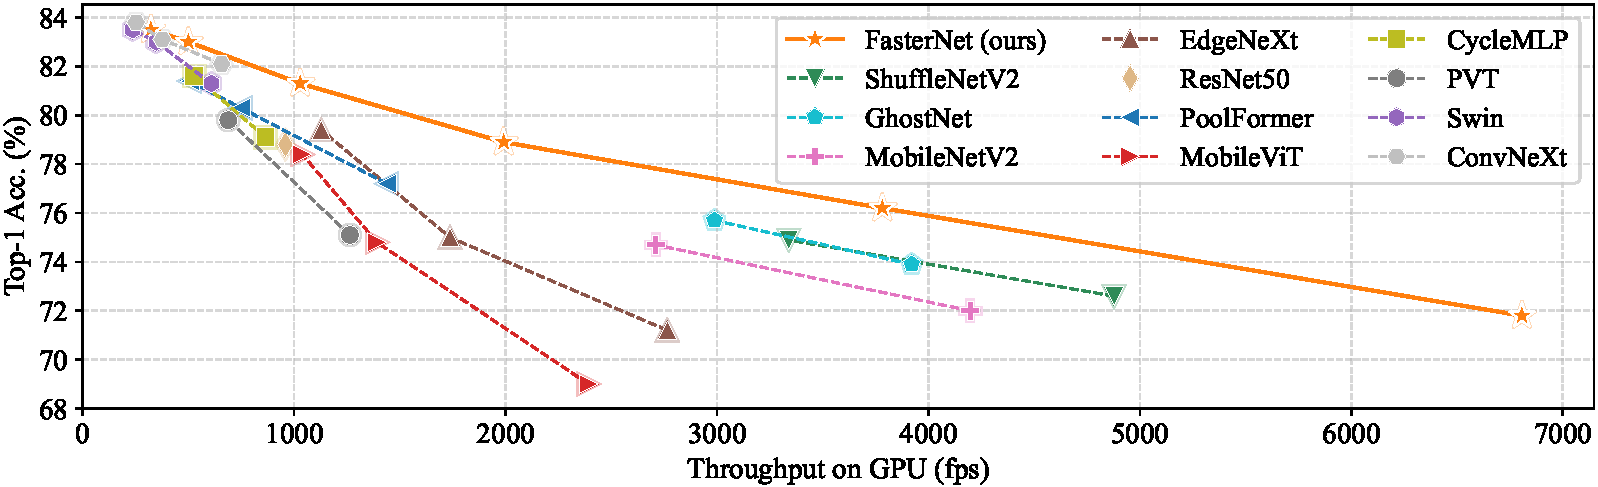
\includegraphics[width=1.\linewidth]{figures/fps_latency_gpu-cropped.pdf}

    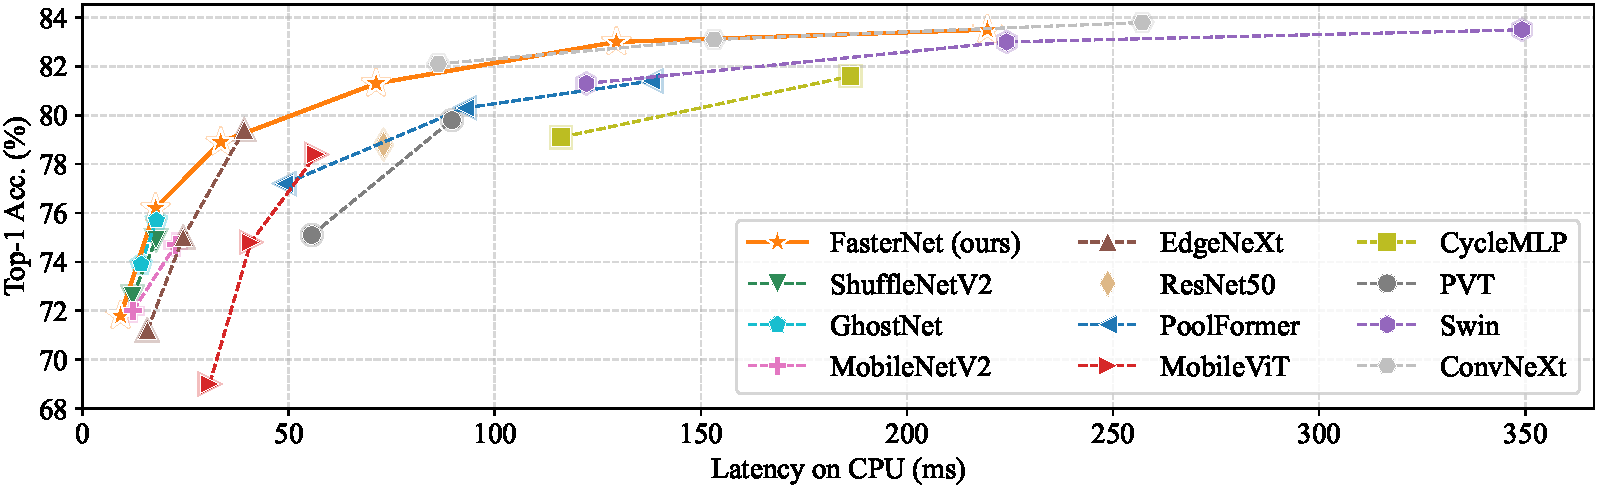
\includegraphics[width=1.\linewidth]{figures/acc_latency_cpu-cropped.pdf}
    
    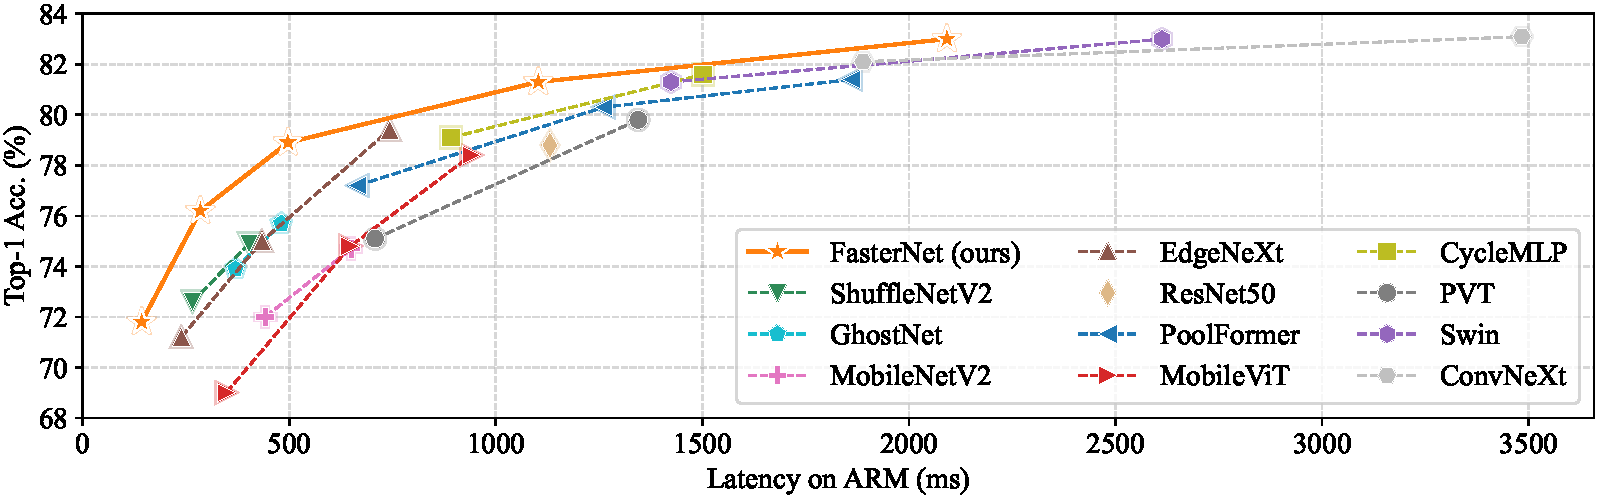
\includegraphics[width=1.\linewidth]{figures/acc_latency_arm-cropped.pdf}
    
    \vspace{-0.1in}
    \caption{Comparison of FasterNet with state-of-the-art networks. FasterNet consistently achieves better accuracy-throughput (the top plot) and accuracy-latency (the medium and bottom plots) trade-offs than others.}
    \label{fig:imagenet_full}
\end{figure*}

% \section{Implementation of PConv}
% We provide the PyTorch-based implementation of PConv in~\cref{lst:code}. There are two forward pass choices, namely forward\_slicing and forward\_split\_cat. The forward\_slicing choice writes the convolutional output in place of the input, which is used for faster inference, but not for training, as the in-place operation modifies the gradient computation. By contrast, the forward\_split\_cat choice concatenates the convolutional output with the feature maps untouched, which preserves the intermediate gradient computation and is used for training. \cref{tab:pconv_implementation} shows the speed comparison of these two choices during inference. The forward\_slicing implementation runs faster than the other one, especially for tiny models and more computation-powerful devices, \eg, for FasterNet-T0 on GPU.

\section{More comparisons with related work}
\medskip\noindent\textbf{Improving FLOPS.} \enspace 
There are a few other works~\cite{ding2022scaling_short,xia2022trt_short} also looking into the FLOPS issue and trying to improve it. They generally follow existing operators and try to find their proper configurations, \eg, RepLKNet~\cite{ding2022scaling_short} simply increases the kernel size while TRT-ViT~\cite{xia2022trt_short} reorders different blocks in the architecture. By contrast, this paper advances the field by proposing a novel and efficient PConv, opening up new directions and potentially larger room for FLOPS improvement.

% \clearpage
% Please add the following required packages to your document preamble:
% \usepackage{booktabs}
% \usepackage{graphicx}
\begin{table*}
\centering
\resizebox{.93\linewidth}{!}{%
% \setlength{\tabcolsep}{1pt}
\begin{tabular}{@{}c|c|c|c|c|c|c|c|c|c@{}}
\toprule
Name &
  Output size &
  \multicolumn{2}{c|}{Layer specification} &
  T0 &
  T1 &
  T2 &
  S &
  M &
  L \\ \midrule
Embedding &
  \large{$\frac{h}{4} \times \frac{w}{4}$}&
  \begin{tabular}[c]{@{}c@{}}Conv\_4\_$c$\_4,\\ BN\end{tabular} &
  \# Channels $c$ &
  40 &
  64 &
  96 &
  128 &
  144 &
  192 \\ \midrule
Stage 1 &
  \large{$\frac{h}{4} \times \frac{w}{4}$}&
  $\left[ \text{\begin{tabular}[c]{@{}c@{}}PConv\_3\_$c$\_1\_1/4,\\ Conv\_1\_$2c$\_1,\\ BN, Acti,\\ Conv\_1\_$c$\_1\end{tabular}}  \right] \times b_1 $  &
  \# Blocks $b_1$ &
  1 &
  1 &
  1 &
  1 &
  3 &
  3 \\ \midrule
Merging &
  \large{$\frac{h}{8} \times \frac{w}{8}$}&
  \begin{tabular}[c]{@{}c@{}}Conv\_2\_$2c$\_2,\\ BN\end{tabular} &
  \# Channels $2c$ &
  80 &
  128 &
  192 &
  256 &
  288 &
  384 \\ \midrule
Stage 2 &
  \large{$\frac{h}{8} \times \frac{w}{8}$}&
  $\left[ \text{\begin{tabular}[c]{@{}c@{}}PConv\_3\_$2c$\_1\_1/4,\\ Conv\_1\_$4c$\_1,\\ BN, Acti,\\ Conv\_1\_$2c$\_1\end{tabular}}  \right] \times b_2 $  &
  \# Blocks $b_2$ &
  2 &
  2 &
  2 &
  2 &
  4 &
  4 \\ \midrule
Merging &
  \large{$\frac{h}{16} \times \frac{w}{16}$}&
  \begin{tabular}[c]{@{}c@{}}Conv\_2\_$4c$\_2,\\ BN\end{tabular} &
  \# Channels $4c$ &
  160 &
  256 &
  384 &
  512 &
  576 &
  768 \\ \midrule
Stage 3 &
  \large{$\frac{h}{16} \times \frac{w}{16}$}&
  $\left[ \text{\begin{tabular}[c]{@{}c@{}}PConv\_3\_$4c$\_1\_1/4,\\ Conv\_1\_$8c$\_1,\\ BN, Acti,\\ Conv\_1\_$4c$\_1\end{tabular}}  \right] \times b_3 $  &
  \# Blocks $b_3$ &
  8 &
  8 &
  8 &
  13 &
  18 &
  18 \\ \midrule
Merging &
  \large{$\frac{h}{32} \times \frac{w}{32}$}&
  \begin{tabular}[c]{@{}c@{}}Conv\_2\_$8c$\_2,\\ BN\end{tabular} &
  \# Channels $8c$ &
  320 &
  512 &
  768 &
  1024 &
  1152 &
  1536 \\ \midrule
Stage 4 &
  \large{$\frac{h}{32} \times \frac{w}{32}$}&
  $\left[ \text{\begin{tabular}[c]{@{}c@{}}PConv\_3\_$8c$\_1\_1/4,\\ Conv\_1\_$16c$\_1,\\ BN, Acti,\\ Conv\_1\_$8c$\_1\end{tabular}}  \right] \times b_4 $  &
  \# Blocks $b_4$ &
  2 &
  2 &
  2 &
  2 &
  3 &
  3 \\ \midrule
Classifier &
  $1  \times 1$ &
  \begin{tabular}[c]{@{}c@{}}Global average pool,\\ Conv\_1\_1280\_1,\\ Acti,\\ FC\_1000\end{tabular} &
  Acti &
  GELU &
  GELU &
  ReLU &
  ReLU &
  ReLU &
  ReLU \\ \midrule
\multicolumn{4}{c|}{FLOPs (G)} &
  0.34 &
  0.85 &
  1.90 &
  4.55 &
  8.72 &
  15.49 \\ \midrule
\multicolumn{4}{c|}{Params (M)} &
  3.9 &
  7.6 &
  15.0 &
  31.1 &
  53.5 &
  93.4 \\ \bottomrule
\end{tabular}%
}
\caption{Configurations of different FasterNet variants. ``Conv\_$k$\_$c$\_$s$'' means a convolutional layer with the kernel size of $k$, the output channels of $c$, and the stride of $s$. ``PConv$\_k\_c\_s\_r$'' means a partial convolution with an extra parameter, the partial ratio of $r$. ``FC\_1000'' means a fully connected layer with 1000 output channels. $h \times w$ is the input size while $b_i$ is the number of FasterNet blocks at stage $i$. The FLOPs are calculated given the input size of $224 \times 224$.}
\label{tab:configuration}
\end{table*}
% \input{tables/pconv_implementation.tex}
% \input{tables/pconv_code.tex}
% \clearpage

\medskip\noindent\textbf{PConv vs. GConv.} \enspace 
PConv is schematically equivalent to a modified GConv~\cite{krizhevsky2012imagenet} that operates on a single group and leaves other groups untouched. Though simple, such a modification remains unexplored before. It's also significant in the sense that it prevents the operator from excessive memory access and is computationally more efficient. From the perspective of low-rank approximations, PConv improves GConv by further reducing the intra-filter redundancy beyond the inter-filter redundancy~\cite{haase2020rethinking_short}.

\medskip\noindent\textbf{FasterNet vs. ConvNeXt.} \enspace 
Our FasterNet appears similar to ConvNeXt~\cite{liu2022convnet} after substituting DWConv with our PConv. However, they are different in motivations. While ConvNeXt searches for a better structure by trial and error, we append PWConv after PConv to better aggregate information from all channels. Moreover, ConvNeXt follows ViT to use fewer activation functions, while we intentionally remove them from the middle of PConv and PWConv, to minimize their error in approximating a regular Conv. 

\medskip\noindent\textbf{Other paradigms for efficient inference.} \enspace 
Our work focuses on efficient network design, orthogonal to the other paradigms, \eg, neural architecture search (NAS)~\cite{elsken2019neural}, network pruning~\cite{molchanov2016pruning}, and knowledge distillation~\cite{hinton2015distilling}. They can be applied in this paper for better performance. However, we opt not to do so to keep our core idea centered and to make the performance gain clear and fair.

\medskip\noindent\textbf{Other partial/masked convolution works.} \enspace 
There are several works~\cite{liu2018image,gao2022convmae,liu2022partial} sharing similar names with our PConv. However, they differ a lot in objectives and methods. For example, they apply filters on partial pixels to exclude invalid patches~\cite{liu2018image}, enable self-supervised learning~\cite{gao2022convmae}, or synthesize novel images~\cite{liu2022partial}, while we target at the channel dimension for efficient inference. 

\section{Limitations and future work}
We have demonstrated that PConv and FasterNet are fast and effective, being competitive with existing operators and networks. Yet there are some minor technical limitations of this paper. For one thing, PConv is designed to apply a regular convolution on only a part of the input channels while leaving the remaining ones untouched. Thus, the stride of the partial convolution should always be 1, in order to align the spatial resolution of the convolutional output and that of the untouched channels. Note that it is still feasible to down-sample the spatial resolution as there can be additional downsampling layers in the architecture. 
And for another, our FasterNet is simply built upon convolutional operators with a possibly limited receptive field. Future efforts can be made to enlarge its receptive field and combine it with other operators to pursue higher accuracy.





% % Please add the following required packages to your document preamble:
% \usepackage{booktabs}
% \usepackage{graphicx}
\begin{table*}
\centering
\resizebox{.93\linewidth}{!}{%
% \setlength{\tabcolsep}{1pt}
\begin{tabular}{@{}c|c|c|c|c|c|c|c|c|c@{}}
\toprule
Name &
  Output size &
  \multicolumn{2}{c|}{Layer specification} &
  T0 &
  T1 &
  T2 &
  S &
  M &
  L \\ \midrule
Embedding &
  \large{$\frac{h}{4} \times \frac{w}{4}$}&
  \begin{tabular}[c]{@{}c@{}}Conv\_4\_$c$\_4,\\ BN\end{tabular} &
  \# Channels $c$ &
  40 &
  64 &
  96 &
  128 &
  144 &
  192 \\ \midrule
Stage 1 &
  \large{$\frac{h}{4} \times \frac{w}{4}$}&
  $\left[ \text{\begin{tabular}[c]{@{}c@{}}PConv\_3\_$c$\_1\_1/4,\\ Conv\_1\_$2c$\_1,\\ BN, Acti,\\ Conv\_1\_$c$\_1\end{tabular}}  \right] \times b_1 $  &
  \# Blocks $b_1$ &
  1 &
  1 &
  1 &
  1 &
  3 &
  3 \\ \midrule
Merging &
  \large{$\frac{h}{8} \times \frac{w}{8}$}&
  \begin{tabular}[c]{@{}c@{}}Conv\_2\_$2c$\_2,\\ BN\end{tabular} &
  \# Channels $2c$ &
  80 &
  128 &
  192 &
  256 &
  288 &
  384 \\ \midrule
Stage 2 &
  \large{$\frac{h}{8} \times \frac{w}{8}$}&
  $\left[ \text{\begin{tabular}[c]{@{}c@{}}PConv\_3\_$2c$\_1\_1/4,\\ Conv\_1\_$4c$\_1,\\ BN, Acti,\\ Conv\_1\_$2c$\_1\end{tabular}}  \right] \times b_2 $  &
  \# Blocks $b_2$ &
  2 &
  2 &
  2 &
  2 &
  4 &
  4 \\ \midrule
Merging &
  \large{$\frac{h}{16} \times \frac{w}{16}$}&
  \begin{tabular}[c]{@{}c@{}}Conv\_2\_$4c$\_2,\\ BN\end{tabular} &
  \# Channels $4c$ &
  160 &
  256 &
  384 &
  512 &
  576 &
  768 \\ \midrule
Stage 3 &
  \large{$\frac{h}{16} \times \frac{w}{16}$}&
  $\left[ \text{\begin{tabular}[c]{@{}c@{}}PConv\_3\_$4c$\_1\_1/4,\\ Conv\_1\_$8c$\_1,\\ BN, Acti,\\ Conv\_1\_$4c$\_1\end{tabular}}  \right] \times b_3 $  &
  \# Blocks $b_3$ &
  8 &
  8 &
  8 &
  13 &
  18 &
  18 \\ \midrule
Merging &
  \large{$\frac{h}{32} \times \frac{w}{32}$}&
  \begin{tabular}[c]{@{}c@{}}Conv\_2\_$8c$\_2,\\ BN\end{tabular} &
  \# Channels $8c$ &
  320 &
  512 &
  768 &
  1024 &
  1152 &
  1536 \\ \midrule
Stage 4 &
  \large{$\frac{h}{32} \times \frac{w}{32}$}&
  $\left[ \text{\begin{tabular}[c]{@{}c@{}}PConv\_3\_$8c$\_1\_1/4,\\ Conv\_1\_$16c$\_1,\\ BN, Acti,\\ Conv\_1\_$8c$\_1\end{tabular}}  \right] \times b_4 $  &
  \# Blocks $b_4$ &
  2 &
  2 &
  2 &
  2 &
  3 &
  3 \\ \midrule
Classifier &
  $1  \times 1$ &
  \begin{tabular}[c]{@{}c@{}}Global average pool,\\ Conv\_1\_1280\_1,\\ Acti,\\ FC\_1000\end{tabular} &
  Acti &
  GELU &
  GELU &
  ReLU &
  ReLU &
  ReLU &
  ReLU \\ \midrule
\multicolumn{4}{c|}{FLOPs (G)} &
  0.34 &
  0.85 &
  1.90 &
  4.55 &
  8.72 &
  15.49 \\ \midrule
\multicolumn{4}{c|}{Params (M)} &
  3.9 &
  7.6 &
  15.0 &
  31.1 &
  53.5 &
  93.4 \\ \bottomrule
\end{tabular}%
}
\caption{Configurations of different FasterNet variants. ``Conv\_$k$\_$c$\_$s$'' means a convolutional layer with the kernel size of $k$, the output channels of $c$, and the stride of $s$. ``PConv$\_k\_c\_s\_r$'' means a partial convolution with an extra parameter, the partial ratio of $r$. ``FC\_1000'' means a fully connected layer with 1000 output channels. $h \times w$ is the input size while $b_i$ is the number of FasterNet blocks at stage $i$. The FLOPs are calculated given the input size of $224 \times 224$.}
\label{tab:configuration}
\end{table*}
% \input{tables/pconv_implementation.tex}
% \clearpage
% \input{tables/pconv_code.tex}